\documentclass{article}

%Packages
\usepackage{amsmath}
\usepackage{amstext}
\usepackage{amssymb}
\usepackage{appendix}
\usepackage{coseoul}
\usepackage{enumerate}
\usepackage{graphicx}
\usepackage{import}
\usepackage{lscape}
\usepackage{modular}

\usepackage[pdfpagemode=UseNone,pdfstartview=FitH,colorlinks=true,linkcolor=blue,citecolor=blue,urlcolor=blue]{hyperref}
\usepackage[all]{hypcap}


% General physics constructs
\newcommand{\bra}[1]{\langle #1 |}
\newcommand{\ket}[1]{| #1 \rangle }
\newcommand{\braket}[2]{\langle #1|#2\rangle}
\newcommand{\bbraket}[3]{ \langle #1 | #2 | #3 \rangle }
\newcommand{\norm}[1]{\| #1\|}
\newcommand{\avg}[1]{\left \langle #1 \right \rangle}
\newcommand{\angavg}[1]{\left \langle #1 \right \rangle}
\newcommand{\abs}[1]{\left \lvert #1 \right \rvert}
\newcommand{\VS}{\textit{\textbf{V}}}
\newcommand{\Tr}{\textrm{Tr}}
\renewcommand{\Re}{\textrm{Re}}
\renewcommand{\Im}{\textrm{Im}}
\newcommand{\basis}[1]{\{\ket{#1}\}}

\newcommand{\omegaqubit}{\omega_{10}}

% Figures. Example usage:
% \quickfig{\columnwidth}{my_image}{This is the caption}{fig:my_fig}
\DeclareRobustCommand{\quickfig}[4]{
\begin{figure}
\begin{centering}
\includegraphics[width=#1]{#2}
\par\end{centering}
\caption{#3}
\label{#4}
\end{figure}
}

\DeclareRobustCommand{\quickwidefig}[4]{
\begin{figure*}[h]
\begin{centering}
\includegraphics[width=#1]{#2}
\par\end{centering}
\caption{#3}
\label{#4}
\end{figure*}
}


\begin{document}

\title{Random walk near a cliff}
\author{Daniel Sank}

\maketitle

Consider a random walk starting at $x=0$.
The walker steps either left or right on each step.
The probability of a left step is $p$, while the probability of a right step is $q \equiv 1-p$.
There is a cliff edge just left of $x=0$ so that if the walker ever steps to $x=-1$ he falls off the cliff and the walk is over.
What is the probability that the walk walker falls off the cliff if left to randomly walk indefinitely?


\section{$5^{th}$ grade method}

Denote by $P_0$ the probability that the man falls off the cliff, given that he starts t $x=0$.
On the first step, he can either step left and fall off the cliff (probability $p$), or he can step to $x = 1$ (probability $q$).
If he steps left the walk is over, but if he steps right he is now at the beginning of a similar problem except that his starting position is $x=1$.
Denote the probability that he falls off the cliff, given that he starts at $x=1$ by $P_1$.
Then we have a simple equation \begin{equation}
P_0 = p + qP_1 \, . \end{equation}
Note that $P_0$ is actually just the probability that the man ever arrives one step closer to the cliff.
Therefore, $P_1 = P_0^2$: In order to fall off the cliff starting one step away, he has to first arrive one step closer, and then do the whole process of falling off starting zero steps away.
Thus we get \begin{equation}
P_0 = p + qP_0^2 \, . \end{equation}
Solving this quadratic equation we find
\begin{equation}
P_0
= \frac{1 \pm \sqrt{(1-2p)^2}}{2q}
= \left\{ \begin{array}{c} p/q \\ 1 \end{array} \right. \, .
\end{equation}
Note that for $p > 1/2$ the square root is actually imaginary so the formula we have derived shouldn't work.
Interestingly, the correct answer, as we will see below, is
\begin{equation}
P_0 = \left\{ \begin{array}{c} p/q, \quad p<1/2 \\ 1, \quad p\geq 1/2 \end{array} \right. \, .
\end{equation}


\section{College method}

Use generating functions.
Define $f_{-1,0}(n)$ as the probability that we make our first arrival off the cliff, given that you started zero steps away, after $n$ steps.
Then the probability of falling is $P = \sum_{n=1}^{\infty} f_{-1,0}(n)$.
Defining the z-transform or ``generating function'' as
\begin{equation}
F(z) = \sum_{n=1}^{\infty} z^n f_{-1,0}(n)
\end{equation}
We can write the probability of falling as
\begin{equation}
P = \lim_{z\rightarrow 1}F_{-1,0}(z) \, . \end{equation}
Therefore, computation of $F$ gives the solution.
This is actually a pretty easy computation because the unconstrained generating function $P_{ji}(z)$ comes from a simple binomial expansion and series summation.

\subsection{Calculation}

To calculate $P_{ji}(z)$ we must first compute $p_{ji}(n)$. How do we compute $p_{ji}(n)$? Denote the state of the walker by a ket; if the walker is at point $j$ we write $|j\rangle$. Each iteration of the process can be represented by a linear transformation:\begin{equation}
L|j\rangle=p|j-1\rangle+q|j+1\rangle \end{equation}
In this notation the probability of being on point $j$ after $n$ steps, given that we started on point $i$ is\begin{equation}
p_{ji}(n)=\langle j|L^{n}|i\rangle\end{equation}
Therefore we must compute the matrix elements of $L^{n}$. This is done by diagonalizing $L$. Introduce a new basis $|\phi\rangle$ \begin{equation}
|\phi\rangle=\sum_{j=-\infty}^{\infty}e^{-i2\pi\phi j}|j\rangle \end{equation}
The action of $L$ on the states $|\phi\rangle$ is computed easily\begin{eqnarray*}
L|\phi\rangle & = & \sum_{j}e^{-i2\pi\phi j}\left(p|j-1\rangle+q|j+1\rangle\right)\\
 & = & pe^{-i2\pi\phi}\sum_{j}e^{-i2\pi\phi j}|j\rangle+qe^{i2\pi\phi}\sum_{j}e^{-i2\pi\phi j}|j\rangle\\
 & = & \left(pe^{-i2\pi\phi}+qe^{i2\pi\phi}\right)|\phi\rangle\end{eqnarray*}
Therefore $|\phi\rangle$ are eigenvectors of $L$. Now we can compute $p_{jk}(n)$ \begin{align}
p_{jl}(n) & = \bbraket{j}{L^n}{l} \\
& = \int_{\phi} \int_{\eta} \braket{j}{\phi} \bbraket{\phi}{L^n}{\eta} \braket{\eta}{l} d\phi d\eta \\
& = \int_{\phi}\int_{\eta}e^{-i 2 \pi j \phi} \delta(\phi-\eta)
\left(p e^{-i 2 \pi \phi} + q e^{i 2 \pi \phi} \right)^{n}
e^{i 2 \pi \eta l} d\phi d\eta \\
& = \int_{\phi} e^{i 2 \pi (l-j)\phi}
\left(p e^{-i2\pi\phi} + q e^{i 2 \pi \phi} \right)^{n} d\phi \\
& = \sum_{k=0}^{n} \binom{n}{k} \int_{\phi} e^{i 2 \pi (l-j) \phi} p^{k} q^{n-k} e^{i 2 \pi (n-2k) \phi} \\
& = \sum_{k=0}^{n} \binom{n}{k} \, p^{k}q^{n-k}\delta_{k,(l-j+n)/2}\\
& = p^{\left(n-(j-l)\right)/2} q^{\left(n+(j-l)\right)/2}\frac{n!}{\left(\frac{n-(j-l)}{2}\right)!\left(\frac{n+(j-l)}{2}\right)!}\end{align}
If we denote the distance traveled $j-l$ by $\Delta$ we can re-express
this as \begin{equation}
p_{\Delta}(n)=p^{(n-\Delta)/2}q^{(n+\Delta)/2}\frac{n!}{\left(\frac{n-\Delta}{2}\right)!\left(\frac{n+\Delta}{2}\right)!} \end{equation}
Note that this expression is only valid when $n$ and $\Delta$ are either both even or both odd. Otherwise $p_{\Delta}(n)$ is zero.

Note also that we could have gotten this answer by a little bit of thinking about combinations of left and right steps. We included this overly complex calculation as a reference for cases with the combinatorics are not obvious.

\subsection{Compute $P_{-1}(z)$}

Because of the translational symmetry, instead of writing $P_{-1,0}(z)$ we can just write $P_{-1}(z)$ for the generating function corresponding to taking one step toward the cliff. When $\Delta$ is odd we can write it generally as $\Delta=2\delta+1$ where $\delta$ is an integer. Since the sum over $n$ will contain only terms where $n$ is odd, we can write $n=2m+1$ and sum over all integers $m$. This gives us\begin{eqnarray*}
P_{n\textrm{ odd}}(z) & = & \sum_{m=0}^{\infty}z^{2m+1}p^{(2m+1-2\delta-1)/2}q^{(2m+1+2\delta+1)/2}\frac{(2m+1)!}{\left(\frac{2m+1-2\delta-1}{2}\right)!\left(\frac{2m+1+2\delta+1}{2}\right)!}\\
 & = & \sum_{m=0}^{\infty}z^{2m+1}p^{m-\delta}q^{m+\delta+1}\frac{\Gamma(2m+2)}{\Gamma(m-\delta+1)\Gamma(m+\delta+2)}\end{eqnarray*}
In the case where $\Delta=-1$ we have $\delta=-1$ and therefore\begin{eqnarray*}
P_{-1}(z) & = & zp\sum_{m=0}^{\infty}\left(pqz^{2}\right)^{m}\frac{\Gamma(2m+2)}{\Gamma(m+2)\Gamma(m+1)}\\
 & = & \frac{1}{2qz}\frac{1-\sqrt{1-4pqz^{2}}}{\sqrt{1-4pqz^{2}}}\end{eqnarray*}

\subsection{Compute $P_{0}(z)$}

When $\Delta$ is even we can write it generally as $\Delta=2\delta$
where $\delta$ is an integer. Since the sum over $n$ contains only
terms where $n$ is even, we can write $n=2m$ and sum over all integers
$m$. This gives us\begin{eqnarray*}
P_{n\textrm{ even}}(z) & = & \sum_{m=0}^{\infty}z^{2m}p^{(2m-2\delta)/2}q^{(2m+2\delta)/2}\frac{(2m)!}{(m-\delta)!(m+\delta)!}\\
 & = & \sum_{m=0}^{\infty}z^{2m}p^{m-\delta}q^{m+\delta}\frac{\Gamma(2m+1)}{\Gamma(m-\delta+1)\Gamma(m+\delta+1)}\end{eqnarray*}
In the present case where $\Delta=0$ we have $\delta=0$ and therefore\begin{eqnarray*}
P_{0}(z) & = & \sum_{m=0}^{\infty}(pqz^{2})^{m}\frac{\Gamma(2m+1)}{\Gamma(m+1)\Gamma(m+1)}\\
 & = & \frac{1}{\sqrt{1-4pqz^{2}}}\end{eqnarray*}

\subsection{Compute $F_{-1}(z)$}

Combining results we get\begin{eqnarray*}
F_{-1}(z) & = & P_{-1}(z)/P_{0}(z)\\
 & = & \frac{1-\sqrt{1-4pqz^{2}}}{2qz}\end{eqnarray*}
Putting in the fact that $q=1-p$ we get \begin{equation}
F_{-1}(z)=\frac{1-\sqrt{1-4p(1-p)z^{2}}}{2(1-p)z} \end{equation}
The probability of absorbtion is $F_{-1}(1)$ so\begin{eqnarray*}
\textrm{absorbtion probability} & = & \frac{1-\sqrt{1-4p(1-p)}}{2(1-p)}\\
 & = & \frac{1-\sqrt{1-4p+4p^{2}}}{2(1-p)}\\
 & = & \frac{1-2\sqrt{(p-1/2)^{2}}}{2(1-p)}\end{eqnarray*}
If $p<1/2,$ the expression in parenthesis under the square root is negative, and taking the square root of the square results in $\emph{minus}$ the the stuff in parenthesis. If $p>1/2$ then we get $\emph{plus}$ the stuff in parenthesis. Therefore \begin{equation}
\textrm{absorbtion probability}=\begin{cases}
\frac{1+2(p-1/2)}{2(1-p)}=\frac{p}{1-p} & \quad p<1/2\\
\frac{1-2(p-1/2)}{2(1-p)}=1 & \quad p>1/2\end{cases} \end{equation}
This function is plotted in Figure 1.

An amazing result of this method is that the two regions for $p<1/2$ and $p>1/2$ come out naturally.

\begin{figure}
\begin{centering}
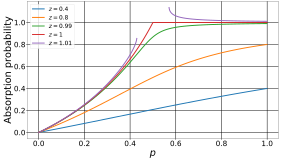
\includegraphics[scale=1.2]{cliff.pdf}
\par\end{centering}
\caption{Absorbtion probability as a function of the probability $p$ of a
leftward step}
\end{figure}


\end{document}